\documentclass[onecolumn, draftclsnofoot,10pt, compsoc]{IEEEtran}
\usepackage{graphicx}
\usepackage{url}
\usepackage{setspace}
\usepackage{caption}
\graphicspath{ {/} }
\usepackage{geometry}
\usepackage{imakeidx}
\makeindex[columns=1, options=-s lou3.ist]
\geometry{textheight=9.5in, textwidth=7in}

% 1. Fill in these details
\def \CapstoneTeamName{   The Visionaries}
\def \CapstoneTeamNumber{   3}
\def \GroupMemberOne{     Kien Tran}
\def \GroupMemberTwo{       Brian Wiltse}
\def \CapstoneProjectName{    Code3 Visionary}
\def \CapstoneSponsorCompany{ Levrum Data Technologies}
\def \CapstoneSponsorPerson{  Carl Niedner}

% 2. Uncomment the appropriate line below so that the document type works
\def \DocType{    
        Requirements Document
        %Technology Review
        %Design Document
        %Progress Report
        }
      
\newcommand{\NameSigPair}[1]{\par
\makebox[2.75in][r]{#1} \hfil   \makebox[3.25in]{\makebox[2.25in]{\hrulefill} \hfill    \makebox[.75in]{\hrulefill}}
\par\vspace{-12pt} \textit{\tiny\noindent
\makebox[2.75in]{} \hfil    \makebox[3.25in]{\makebox[2.25in][r]{Signature} \hfill  \makebox[.75in][r]{Date}}}}
% 3. If the document is not to be signed, uncomment the RENEWcommand below
%\renewcommand{\NameSigPair}[1]{#1}

%%%%%%%%%%%%%%%%%%%%%%%%%%%%%%%%%%%%%%%
\begin{document}

\begin{titlepage}
    \pagenumbering{gobble}
    \begin{singlespace}
      
\includegraphics[height=4cm]{coe_v_spot1}
        \hfill 
        % 4. If you have a logo, use this include graphics command to put it on the cover sheet.
        %\includegraphics[height=4cm]{CompanyLogo}   
        \par\vspace{.2in}
        \centering
        \scshape{
            \huge CS Capstone \DocType \par
            \large{Spring Term}\par
            {\large\today}\par
            \vspace{.5in}
            \textbf{\Huge\CapstoneProjectName}\par
            \vfill
            {\large Prepared for}\par
            \Huge \CapstoneSponsorCompany\par
            \vspace{5pt}
            {\Large\NameSigPair{\CapstoneSponsorPerson}\par}
            {\large Prepared by }\par
            Group\CapstoneTeamNumber\par
            % 5. comment out the line below this one if you do not wish to name your team
            %\CapstoneTeamName\par 
            \vspace{5pt}
            {\Large
                \NameSigPair{\GroupMemberOne}\par
                \NameSigPair{\GroupMemberTwo}\par
            }
            \vspace{20pt}
        }
        \begin{abstract}
                Optimal placement of emergency resources is critical to ensuring public safety.
                However, anticipating demand for emergency resources is a challenge for city and county planners. 
                The Code3 Visionary (C3V) project will utilize machine learning combined with statistical analysis to predict future patterns of emergency demand. 
                C3V will require obtaining and preparing data for analysis, training a machine learning algorithm, running analyses, and providing the results of the analyses to users via an API.
                Each of these components will be completed as separate modules.
                This document describes the requirements for each module.
        \end{abstract}
    \end{singlespace}
\end{titlepage}
\newpage
\pagenumbering{arabic}
\tableofcontents
% 7. uncomment this (if applicable). Consider adding a page break.
%\listoffigures
%\listoftables
\clearpage

% 8. now you write!
\section{Introduction}
    \subsection{Purpose}
    % This subsection should
    % a) Delineate the purpose of the Software Requirement Specification (SRS);
    % b) Specify the intended audience for the SRS.
    The purpose\index{purpose} of this requirements document is to identify requirements of the Code3 Visionary Project. 
    The intended audience\index{audience} is the Senior Capstone course professors and the sponsored company, Levrum. 
    Levrum is a start up in its early stages; as such, many of the requirements and implementation details will be informed by research into best practices into relevant fields, such as statistical analysis, machine learning, artificial intelligence, and availability of various types of data.
    
    \subsection{Scope}
    % This subsection should
    % a) Identify the software product(s) to be produced by name (e.g., Host DBMS, Report Generator, etc.);
    % b) Explain what the software product(s) will, and, if necessary, will not do;
    % c) Describe the application of the software being specified, including relevant benefits, objectives, and
    % goals;
    % d) Be consistent with similar statements in higher-level specifications (e.g., the system requirements
    % specification), if they exist.
    
    Code3 Visionary will generate a predictive model of emergency incident types and density at a given time and place. 
    The predictive model will utilize machine learning to select the features that appear to have the greatest correlation with specific types of incidents. 
    The goal is to be able to generate the predicted number of calls of a given type, given a cause, place, year, and some knowledge of an area's demographics and geographic features.
    Users will be able access the predicted number of calls through an application programming interface (API) \index{API} and pass it the three values (location, call type, year) to receive the number.
    
    Additionally, Code3 Visionary's API will be used by Levrum's existing employees who will collect the number of calls to create a predicted set of calls for the city of Charlotte, North Carolina.
    This call set can then be used in Levrum's existing tool, Code3 Strategist\index{Code3 Strategist}, which generates what-if analysis\index{analysis!what-if} of what would happen based on hypothetical call volumes and locations. 
    %Users will be able to use predicted call data, as input into the Code3 Strategist\index{Code3 Strategist} simulation software. \par
    All components of C3V will be applied and tested for the case of Levrum's client, Charlotte, NC.
    Variation in data types and formats will require adjustment of C3V's tools.
    A stretch goal of the project is to make the tools generalized and create test cases to verify their accuracy for other cities in the United States.
    
    \subsection{Definitions, acronyms, and abbreviations}
    % This subsection should provide the definitions of all terms, acronyms, and abbreviations required to properly
    % interpret the SRS. This information may be provided by reference to one or more appendixes in the SRS or
    % by reference to other documents
        \begin{itemize}
            \item\textbf{C3V}. Code 3 Visionary
            \item\textbf{EMS}. Emergency Medical Services.
            \item\textbf{What-if analysis}. A feature of Code3 Strategist, Levrum's existing software, that allows a user to run hypothetical scenarios against current or planned resource allocations.  
        \end{itemize}
    \subsection{References}
    % This subsection should
    % a) Provide a complete list of all documents referenced elsewhere in the SRS;
    % b) Identify each document by title, report number (if applicable), date, and publishing organization;
    % c) Specify the sources from which the references can be obtained.
    No current references.
    \subsection{Overview}
    % This subsection should
    % a) Describe what the rest of the SRS contains;
    % b) Explain how the SRS is organized.
    The following sections contain the requirements, functionality, and constraints of Code3 Visionary. Section 2 contains an overall description of Code3 Visionary which includes the different pieces that makes up C3V as well as the logistics and time estimation of C3V's development. Section 3 details specific requirements. Following Section 3 is an index of keywords.

\section{Overall Description}
    \subsection{Product Perspective}
    
    % This subsection of the SRS should put the product into perspective with other related products. If the product
    % is independent and totally self-contained, it should be so stated here. If the SRS defines a product that is a
    % component of a larger system, as frequently occurs, then this subsection should relate the requirements of
    % that larger system to functionality of the software and should identify interfaces between that system and the
    % software.
    % A block diagram showing the major components of the larger system, interconnections, and external interfaces
    % can be helpful.
    
    The Code3 Visionary (C3V) project is an independent product. 
    However, C3V is not considered completely self-contained due to its interaction with Levrum's previous project, Code3 Strategist.
    A stretch goal will be to have output from C3V in a format that is compatible with Code3 Strategist.
    The following is a block diagram showing the major components that make up Code3 Visionary:\\
    \begin{figure}[h!]
        \centering
        \includegraphics[height=10cm, width=17cm]{Code3VisionaryDiagram.eps}
        \caption{Diagram of the Code3 Visionary}
        \label{fig:diagram}
    \end{figure}
    
    % This subsection should also describe how the software operates inside various constraints. For example,
    % these constraints could include
    % a) System interfaces;
    % b) User interfaces;
    % c) Hardware interfaces;
    % d) Software interfaces;
    % e) Communications interfaces;
    % f) Memory;
    % g) Operations;
    % h) Site adaptation requirements.
    The work flow of C3V begins at the top-left of Figure \ref{fig:diagram}.
    Data will first be gathered, explored, and transformed into a useful format for analysis via a command-line interface. 
    All of the data will then be input into a genetic algorithm that selects a subset of features from the data and maximizes an adjusted R-squared value as its objective.
    The adjusted R-squared value will be generated by running a geographically weighted regression (GWR) on the selected features and a given incident type.
    The GWR with the highest adjusted R-squared value will be C3V's trained model.
    Using zoning and demographic projections for future years, C3V will store the predicted number of each type of call in an API, which can be used by Levrum or other authorized users. 
    %The goal for this project is a minimal user interface
    %A web form that will show a map with outlined cities on the map.
    %Users will only need to supply location and year to receive a predictive output by the system.
    %This output will be in the form of heat maps, realistic call data set (forecast horizon), and generated accuracy metrics.
    
    \subsection{Product Functions}
    The following user stories illustrate the desired functionality of Code3 Visionary. Estimated time to complete each story is included.
    \begin{itemize}
        \item{User Story 1:}\index{user stories} As a user, I want a tool that retrieves and compiles data for a target area into a complete data set that is ready for analysis. The resulting data set should include:
        \begin{itemize}
            \item Census demographics, which will be retrieved directly from the Census API.
            \item Zoning information, which will be locally available.
            \item Number of each type of emergency call, which will be locally available.
        \end{itemize}
        Expected time to complete for Brian: 20 weeks for a total of 200 person hours.
        \item{User Story 2:} As a user, I want Code3 Visionary to generate a predictive model with the highest adjusted R-squared value, relative to other models. I want documentation to show a comparison of the adjusted R-squared value between at least the following models:
        \begin{itemize}
            \item Best guess of features to include
            \item Model predicting the best features automatically
        \end{itemize}
        Expected time to complete for Kien: 8 weeks for a total of 32 person hours.
        \item{User Story 3:} As a user, I want Code3 Visionary's results to be accessible through an API, so that the results can be used in other software like Code3 Strategist. I want the API to be able to generate the number of calls I can expect at a given time, place, causality. 
        
        Expected time to complete for Kien: 2 weeks for a total of 8 person hours.
    \end{itemize}
    
    \subsection{User Characteristics}\index{characteristics!users}
    % This subsection of the SRS should describe those general characteristics of the intended users of the product
    % including educational level, experience, and technical expertise. It should not be used to state specific
    % requirements, but rather should provide the reasons why certain specific requirements are later specified in
    % Section 3 of the SRS.
    The users of Code3 Visionary will be software engineers at Levrum.
    Engineers will use the data transformation tool to generate shapefiles needed for analysis, perform analysis, and use the API to generate a set of predicted calls.
    As software engineers, C3V's users will be highly technical.
    The API may be used by authorized users outside Levrum, but they can be expected to have at least moderate technical skills.
    \subsection{Constraints}
    % This subsection of the SRS should provide a general description of any other items that will limit the developer’s
    % options. These include
    % a) Regulatory policies;
    % b) Hardware limitations (e.g., signal timing requirements);
    % c) Interfaces to other applications;
    % d) Parallel operation;
    % e) Audit functions;
    % f) Control functions;
    % g) Higher-order language requirements;
    % h) Signal handshake protocols (e.g., XON-XOFF, ACK-NACK);
    % i) Reliability requirements;
    % j) Critically of the application;
    % k) Safety and security considerations.
     
    C3V's primary constraint\index{constraints} will be the availability and robustness of data. 
    Since the U.S. Census is an estimation based off of user input, the data that is gathered for the baseline and prediction will be dependent on the people who took the survey.
    Furthermore, Census data will account for residential areas only. 
    Demographics from the Census will be missing in areas where there are no residential housing.
    Useful data beyond what is obtained from the Census will likely be obtained from city or county staff, and this amount and quality of data available will vary.
    
    Another important constraint is the predictive power of regression models. C3V will predict emergency incident density based on features that appear to correlate most with emergency incidents; however, correlation does not imply causation. C3V's results should ideally be combined with other methods of prediction.
    
    \subsection{Assumptions and Dependencies}\index{dependencies}
    % This subsection of the SRS should list each of the factors that affect the requirements stated in the SRS.
    % These factors are not design constraints on the software but are, rather, any changes to them that can affect
    % the requirements in the SRS. For example, an assumption may be that a specific operating system will be
    % available on the hardware designated for the software product. If, in fact, the operating system is not available,
    % the SRS would then have to change accordingly. 
    \begin{figure}[h!]
        \centering
        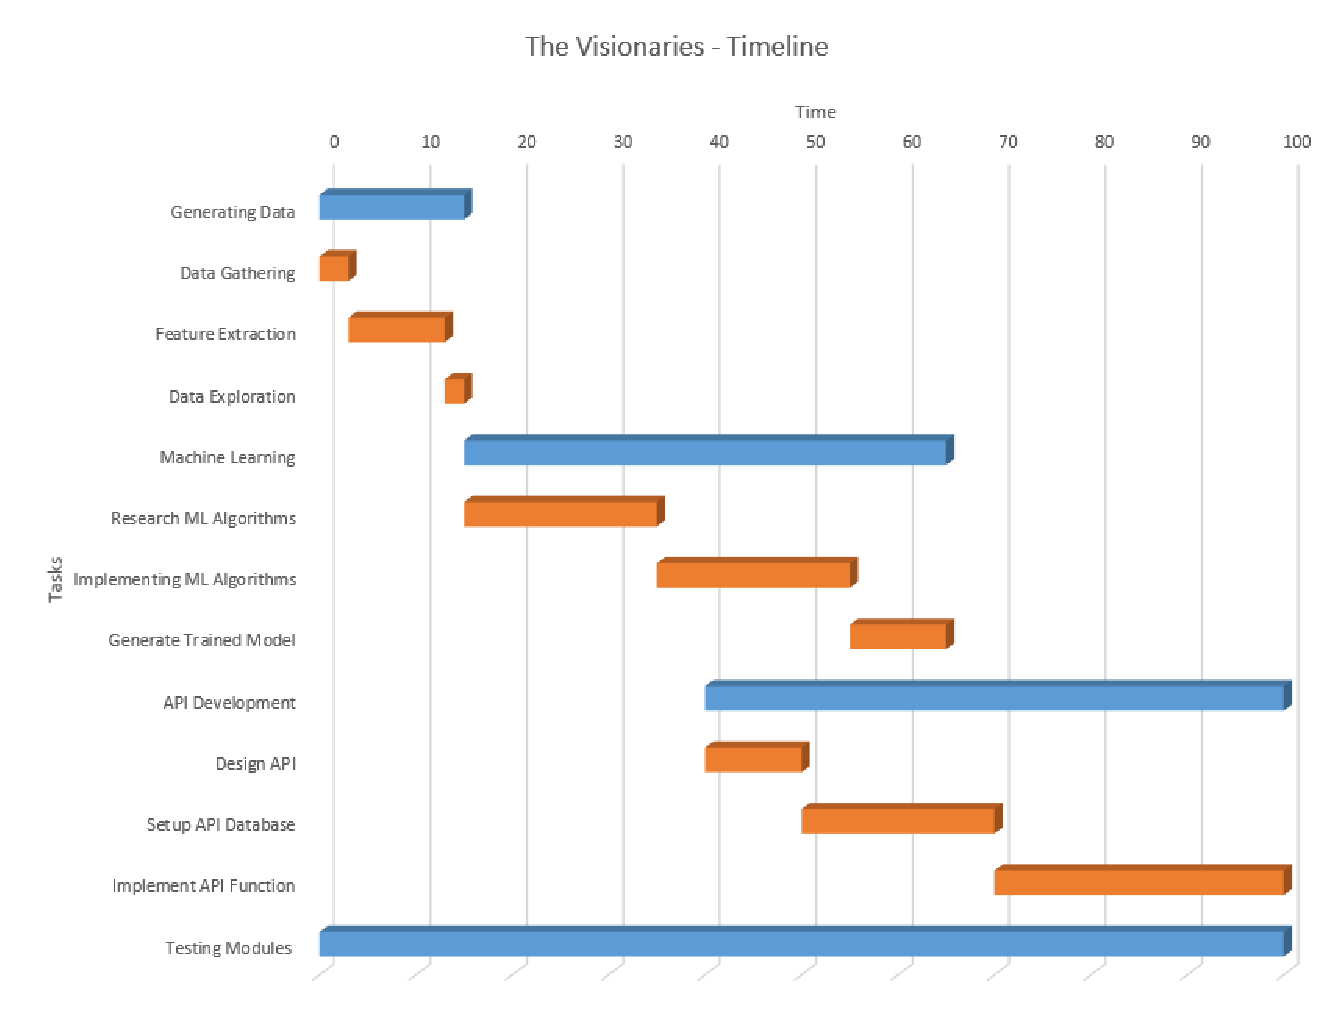
\includegraphics[height=10cm, width=17cm]{Timeline.eps}
        \caption{Gantt Chart of Project Dependencies}
        \label{fig:timeline}
    \end{figure}
    The Code3 Visionary project assumes that it is possible to generate a reliable predictive model of emergency incidents. Specifically, it depends upon:
    
    \begin{itemize}
    \item Availability of public-domain data.
    \item APIs that allow automatic retrieval of those data.
    \item A machine learning algorithm that can generate the best feature that correlates with the call set given the available data.
    \end{itemize}
    
    \subsection{Apportioning of Requirements}
    % This subsection of the SRS should identify requirements that may be delayed until future versions of the system.
    The current iteration of Code3 Visionary will consist mainly of creating tools for obtaining and transforming data, running analyses on the data, implementing a machine learning algorithm to select features from the obtained data, and building an API to store and return the results of our resulting model.
    Development of a user interface and updating Code3 Strategist to utilize the functionality of Code3 Visionary will be addressed in future versions of the project.
    
\section{Specific Requirements}
    \subsection {External Interfaces}\index{user interface}
    C3V will consist of three interfaces. One interface will compile and transform data into a form appropriate for analysis. Another interface will utilize that generated data set to select the best features to make predictions. Finally, an API will store and retrieve the prediction results.
    Both the data ingestion and the machine learning tools will be internal interfaces, consisting of command-line tools that will be used by Levrum's software and data engineers.
    The API will be an external interface, into which the user will input a cause, location, and year to receive the number of predicted calls based on C3V's predictive model.
    
    \subsection{Functions}
    \begin{itemize}
        \item The system shall ingest data from public domain sources and local data sets retrieved from Levrum's clients.
        The sources of data used by the current iteration of C3V are:
        \begin{itemize}
            \item United States Census (public)
            \item Zoning (provided by client)
            \item Traffic analysis zone (provided by client)
            \item Incident logs (provided by client)
        \end{itemize}
        \item The system shall allow users to insert arbitrary sets of features from ingested data, which will be used to generate a predictive model for the number of emergency calls for an arbitrary incident type.
        Some features will be extracted as-is; however, others will require further conditioning. For example, the population of an area is provided by the Census, but population density is anticipated to be an important feature for our predictive model. The population density feature for a given zone can be calculated given the population and area of the zone.
        \item Stretch goal: The system shall be usable by Code3 Strategist via API calls that can provide Code3 Visionary's predictive model as an input to what-if analyses.
    \end{itemize}
    
    \subsection{Performance Requirements}\index{performance}
    Performance metrics are not a concern at this time; however, care will be taken to make the system as performant as possible, in accordance with good software engineering practice. 
    Performance optimization will be addressed in future iterations of the project. 
    
    \subsection{Logical Database Requirements}
    C3V's current priority is developing a work flow for generating a predictive model and applying it to Charlotte, NC.
    Data will currently be stored locally on the user's machine.
    
    \subsection{Design Constraints}\index{constraints}
    Code3 Visionary's scope does not involve creating new algorithms for machine learning or artificial intelligence.
    As a result, we will be limited by the effectiveness of current implementations of machine learning and artificial intelligence algorithms.
    Given the complexity of some machine learning algorithms, hardware constraints may be an issue in future iterations; however no current feature of C3V exceeds the capabilities of available hardware.
    
    \subsection{Software System Attributes}\index{software attributes}
    \begin{itemize}
    \item \textbf{Accuracy.} The system shall demonstrate with unit or integration tests that data is being transformed and aggregated correctly.
    \item \textbf{Testability.}\index{testing} The system shall be modular enough to allow testing for each major step of data collection: 
        \begin{itemize}
            \item Obtaining and appending Census data
            \item Appending incident counts
            \item Appending zoning data
            \item Areal interpolation
            \item Data transformations
            \item Feature extraction
        \end{itemize}
    \item \textbf{Adaptability.} The system shall be able to generate a shapefile with U.S. Census demographics for an arbitrary county in the United States. 
    \item \textbf{Extensibilty and Modifiability.} The system shall use a pipeline structure, so that more data can be added to final shapefile by creating a new data collection module and inserting the new module into the pipeline. 
    \item \textbf{Configurability}. The genetic algorithm module shall be capable of adding and removing features as needed to improve each model's R-squared value.
    \end{itemize}
    
\printindex

    
\end{document}
